\chapter{Eigenzeit, Zeitdilatation und Längenkontraktion}

Wir wählen oft Einheiten, in denen die Lichtgeschwindigkeit $c=1$ beträgt. In diesen Einheiten lassen sich ein Jahr Zeit und ein Lichtjahr Entfernung direkt miteinander vergleichen, und die Formeln sind viel leichter zu lesen. Wo $c$ physikalisch eine Rolle spielt, setzen wir es wieder ein. Eine Dimensionsanalyse genügt, um seinen Platz zu bestimmen.

\section{Das galileische Raumzeitgitter}

Beginnen wir mit der Beziehung aus der Zeit vor Einstein zwischen einem ruhenden Bezugssystem und einem Zug, der sich mit der Geschwindigkeit $v$ entlang der $x$-Achse bewegt:
\begin{align}
x' &= x-vt, & t'&=t.
\label{eq:l4-galilean}
\end{align}
Die zweite Gleichung enthält Newtons Annahme einer universellen Zeit. Alle Beobachter verwenden dieselben Gleichzeitigkeitsflächen, obwohl sich ihre räumlichen Ursprünge relativ zueinander bewegen.

Der ungestrichene Beobachter stehe neben der Strecke, der gestrichene fahre im Zug. Der Ursprung des Zuges hat $x'=0$; seine Weltlinie in den ungestrichenen Koordinaten lautet daher
\begin{equation}
x=vt.
\end{equation}
Diese schräge Gerade ist die $t'$-Achse. Im Gegensatz dazu besagt $t'=t$, dass alle Linien mit konstantem $t'$ dieselben horizontalen Linien sind wie die mit konstantem $t$.

\begin{figure}[H]\centering
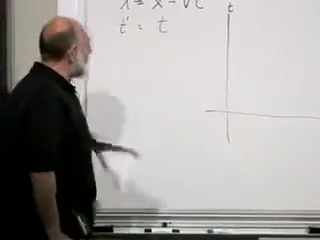
\includegraphics[width=0.72\textwidth]{lecture_04_figure_02.png}\caption{Die galileische Transformation und das anfängliche $t$-$x$-Gitter. Der bewegte Ursprung zeichnet $x=vt$ nach, während die beiden Bezugssysteme gemeinsame Linien konstanter Zeit behalten.}\lectureframe{00:03:06}\end{figure}

Löst man Gl.~\eqref{eq:l4-galilean} nach den ungestrichenen Koordinaten auf, erhält man
\begin{align}
x&=x'+vt'=x'+vt, & t&=t'.
\end{align}
Die inverse Transformation hat dieselbe Form, wenn man $v$ durch $-v$ ersetzt. Bewegt sich der Zug relativ zum Bahnhof vorwärts, so bewegt sich der Bahnhof relativ zum Zug rückwärts. Diese Reziprozität bleibt in der speziellen Relativitätstheorie erhalten, die universelle Zeit jedoch nicht.

\section{Die Lorentz-Korrektur}

Galileische Transformationen können nicht dafür sorgen, dass die Lichtgeschwindigkeit in allen Inertialsystemen gleich ist. Die korrigierten Beziehungen lauten, zunächst in Einheiten mit $c=1$,
\begin{align}
x'&=\frac{x-vt}{\sqrt{1-v^2}}, &
t'&=\frac{t-vx}{\sqrt{1-v^2}}.
\label{eq:l4-lorentz-natural}
\end{align}
Mit den üblichen Einheiten ergibt sich
\begin{align}
x'&=\frac{x-vt}{\sqrt{1-v^2/c^2}}, &
t'&=\frac{t-vx/c^2}{\sqrt{1-v^2/c^2}}.
\label{eq:l4-lorentz-c}
\end{align}

\begin{figure}[H]\centering
\includegraphics[width=0.74\textwidth]{lecture_04_figure_05.png}\caption{Die Lorentz-Transformation mit wieder eingesetzten Faktoren von $c$.}\lectureframe{00:09:10}\end{figure}

Für $v\ll c$ sind sowohl $v^2/c^2$ als auch $vx/c^2$ unter den Bedingungen, unter denen die Newtonsche Mechanik verwendet wird, sehr klein. Gleichung~\eqref{eq:l4-lorentz-c} geht dann in das galileische Ergebnis über. Die Relativitätstheorie verwirft die Newtonsche Kinematik nicht, sondern bestimmt ihren Gültigkeitsbereich.

Bei $v=c$ verschwindet der Nenner. Ein Inertialsystem kann sich relativ zu einem anderen Inertialsystem nicht mit Lichtgeschwindigkeit bewegen. Weit unterhalb dieser Grenze sind die Korrekturen klein; in ihrer Nähe wird die Vermischung von $x$ und $t$ jedoch unvermeidlich.

Die Bewegung wurde entlang $x$ gewählt, daher ändern sich die transversalen Koordinaten nicht:
\begin{equation}
y'=y,\qquad z'=z.
\end{equation}
Warum das so ist, lässt sich folgendermaßen erkennen: Man bringe identische transversale Meterstäbe im Zug und auf dem Bahnsteig an. Ein Beobachter, der sich genau halbwegs zwischen den beiden Bezugssystemen bewegt, sieht die Stäbe mit gleich großen, entgegengesetzten Geschwindigkeiten auf sich zukommen. Nichts an der Anordnung könnte dazu führen, dass einer der beiden transversalen Stäbe kürzer erscheint als der andere.

\section{Lorentz-Transformationen entlang des Lichtkegels}

Gl.~\eqref{eq:l4-lorentz-natural} lässt sich geometrisch deuten. Addiert man die beiden Gleichungen, erhält man
\begin{align}
t'+x'
&=\frac{(t-vx)+(x-vt)}{\sqrt{1-v^2}}\\
&=(t+x)\frac{1-v}{\sqrt{1-v^2}}\\
&=(t+x)\sqrt{\frac{1-v}{1+v}}.
\label{eq:l4-null-plus}
\end{align}
Subtrahiert man sie in der umgekehrten Reihenfolge, ergibt sich
\begin{align}
t'-x'
&=\frac{(t-vx)-(x-vt)}{\sqrt{1-v^2}}\\
&=(t-x)\frac{1+v}{\sqrt{1-v^2}}\\
&=(t-x)\sqrt{\frac{1+v}{1-v}}.
\label{eq:l4-null-minus}
\end{align}

\begin{figure}[H]\centering
\includegraphics[width=0.75\textwidth]{lecture_04_figure_06.png}\caption{Die Lorentz-Transformation, umgeschrieben mit den Nullkombinationen $t+x$ und $t-x$. Ihre Skalierungsfaktoren sind reziprok.}\lectureframe{00:18:45}\end{figure}

Die Kombinationen $t+x$ und $t-x$ sind Koordinaten entlang der beiden lichtartigen Richtungen bei $45^\circ$. Ein Boost staucht eine dieser Richtungen und streckt die andere um den reziproken Faktor. Er dreht keine der beiden aus ihrer Richtung bei $45^\circ$ heraus. Lichtstrahlen bleiben daher Lichtstrahlen – so zeigt sich die Invarianz der Lichtgeschwindigkeit im Raumzeitbild.

\begin{classroomqa}\audiencequestion{Der halbwegs zwischen den Bezugssystemen bewegte Beobachter sieht ein symmetrisches Experiment. Wie lässt sich daraus aber das Ergebnis für die Beobachter im Zug und auf dem Bahnsteig ableiten?\lecturetimestamp{00:20:48}}\lecturerresponse{Dabei wird eine weitere Tatsache vorausgesetzt: Das Zusammenfallen von Ereignissen ist invariant. Treffen die Enden der Stäbe aufeinander, ist dieses Treffen ein einzelnes Raumzeitereignis. Jeder Inertialbeobachter kann ihm andere Koordinaten zuweisen, doch keiner kann ein einziges Zusammentreffen in zwei verschiedene Orte aufspalten. Lichtblitze, die dort ausgesandt werden, wo die entsprechenden Enden zusammentreffen, machen diese Ereignisse beobachtbar. Die Symmetrie im halbwegs bewegten Bezugssystem und die Invarianz der beiden Zusammentreffen an den Enden zeigen, dass die transversalen Längen gleich sind.}\end{classroomqa}

\begin{classroomqa}\audiencequestion{Muss sich der Radfahrer, der das halbwegs bewegte Bezugssystem repräsentiert, tatsächlich in der Mitte zwischen den Stabenden befinden?\lecturetimestamp{00:22:25}}\lecturerresponse{Nein. Ein Bezugssystem ist ein ganzes Netz von Beobachtern und Uhren, nicht ein einzelnes Auge an einem bestimmten Ort. Der Radfahrer kann die Lichtblitze von den Stabenden später empfangen und erschließen, wo sie ausgesandt wurden. Entscheidend ist der Ort jedes Aussendeereignisses in der Raumzeit, nicht der Ort, an dem das Licht schließlich empfangen wird.}\end{classroomqa}

Die Zusammensetzung aufeinanderfolgender Geschwindigkeiten ist eine weitere Folge derselben Transformation, wird aber bewusst der nächsten Vorlesung überlassen. Hier geht es zunächst darum, die invariante Größe zu bestimmen, die eine bewegte Uhr misst.

\section{Das invariante Intervall}

Bei einer Drehung gewöhnlicher kartesischer Achsen bleibt die Größe $x^2+y^2$ unverändert. Lorentz-Transformationen erhalten eine andere quadratische Form. Aus Gl.~\eqref{eq:l4-lorentz-natural} folgt
\begin{align}
t'^2-x'^2
&=\frac{(t-vx)^2-(x-vt)^2}{1-v^2}\\
&=\frac{t^2-2vtx+v^2x^2-x^2+2vtx-v^2t^2}{1-v^2}\\
&=t^2-x^2.
\label{eq:l4-interval}
\end{align}
Die gemischten Terme heben sich auf, und im verbleibenden Zähler lässt sich der gemeinsame Faktor $1-v^2$ ausklammern.

\begin{figure}[H]\centering
\includegraphics[width=0.76\textwidth]{lecture_04_figure_07.png}\caption{Die Herleitung von $t'^2-x'^2=t^2-x^2$ an der Tafel.}\lectureframe{00:33:15}\end{figure}

Mit drei räumlichen Dimensionen lautet die Invariante in Einheiten mit $c=1$
\begin{equation}
t'^2-x'^2-y'^2-z'^2=t^2-x^2-y^2-z^2
\end{equation}
Allgemeiner verwenden wir für zwei Ereignisse Koordinatendifferenzen:
\begin{equation}
\Delta s^2
=c^2\Delta t^2-\Delta x^2-\Delta y^2-\Delta z^2.
\label{eq:l4-spacetime-interval}
\end{equation}
Alle Inertialbeobachter stimmen in diesem Wert überein, auch wenn sie sich über seine getrennten Zeit- und Raumanteile nicht einig sind.

\section{Eigenzeit und bewegte Uhren}

Man stelle sich ein Gitter ruhender Beobachter vor, deren Uhren durch den Austausch von Lichtsignalen synchronisiert wurden. Ihre Anzeigen definieren die Koordinatenzeit $t$. Nun trage man eine Armbanduhr durch dieses Gitter. Ihre eigene Anzeige folgt der Uhr entlang ihrer Weltlinie; diese Anzeige ist die Eigenzeit.

Für zwei zeitartig getrennte Ereignisse definieren wir
\begin{equation}
c^2\Delta\tau^2
=c^2\Delta t^2-\Delta x^2-\Delta y^2-\Delta z^2.
\label{eq:l4-proper-time}
\end{equation}
In einer räumlichen Dimension und mit $c=1$ vereinfacht sich das zu
\begin{equation}
\Delta\tau=\sqrt{\Delta t^2-\Delta x^2}.
\end{equation}
Die Quadratwurzel erinnert an die Formel für einen gewöhnlichen Abstand, doch das Minuszeichen verändert die Geometrie.

Es gibt drei Fälle:
\begin{align}
\Delta t^2-\Delta x^2 &>0 &&\text{timelike},\\
\Delta t^2-\Delta x^2 &=0 &&\text{lightlike},\\
\Delta t^2-\Delta x^2 &<0 &&\text{spacelike}.
\end{align}
Innerhalb des Lichtkegels ist die Eigenzeit reell. Auf dem Lichtkegel, wo $x=\pm t$ gilt, ist sie null, obwohl die Ereignisse nicht zusammenfallen müssen. Ein Lichtstrahl kann genau solche Ereignisse verbinden. Außerhalb des Lichtkegels ist die Trennung raumartig; sie beschreibt man besser durch die reelle Eigenentfernung $\sqrt{\Delta x^2-\Delta t^2}$ als durch eine imaginäre Uhrzeit.

\begin{figure}[H]
\centering
\includegraphics[width=0.73\textwidth]{lecture_04_figure_08.png}

\vspace{0.8em}

\begin{tikzpicture}[x=1.0cm,y=1.0cm]
\draw[->] (-3.3,0) -- (3.3,0) node[right] {$x$};
\draw[->] (0,-0.4) -- (0,4.0) node[above] {$t$};
\draw[thick] (0,0) -- (3.0,3.0) node[above right] {$x=t$};
\draw[thick] (0,0) -- (-3.0,3.0) node[above left] {$x=-t$};
\node at (0,2.0) {timelike};
\node at (2.25,1.05) {spacelike};
\node at (-2.25,1.05) {spacelike};
\end{tikzpicture}\caption{Der Lichtkegel an der Tafel mit einer klaren Einteilung in zeitartige, lichtartige und raumartige Trennungen.}\lectureframe{00:38:40}\end{figure}

Warum entspricht Gl.~\eqref{eq:l4-proper-time} einer Uhrenanzeige? Für eine ruhende Uhr gilt $\Delta x=0$, also $\Delta\tau=\Delta t$. Bei einer gleichförmig bewegten Uhr wählen wir das gestrichene Bezugssystem, in dem diese Uhr ruht. Dort gilt $\Delta x'=0$, und aus der Invarianz folgt
\begin{equation}
\Delta\tau
=\sqrt{\Delta t'^2-\Delta x'^2}
=\Delta t'.
\end{equation}
Bewegte Uhren messen somit die Eigenzeit.

\begin{classroomqa}\audiencequestion{Sind ``das Intervall zwischen den Ereignissen'' und ``die Anzeige der verwendeten Uhr'' zwei Bezeichnungen für dasselbe?\lecturetimestamp{00:44:49}}\lecturerresponse{Sie stimmen überein, wenn eine ideale Uhr sich inertial von einem Ereignis zum anderen bewegt. Das invariante Intervall ist eine geometrische Größe; die Differenz zwischen den Anzeigen der mitbewegten Uhr an den Endpunkten ist ihre physikalische Messung. Eine ruhende Koordinatenuhr zeigt im Allgemeinen ein anderes Koordinatenzeitintervall an.}\end{classroomqa}

\section{Zeitdilatation und Gleichzeitigkeit}

Betrachten wir den Ursprung des bewegten Bezugssystems. Seine Weltlinie erfüllt
\begin{equation}
x'=0,\qquad x=vt.
\end{equation}
Dieselbe schräge Gerade ist sowohl die Bahn der bewegten Uhr als auch die $t'$-Achse.

\begin{figure}[H]\centering
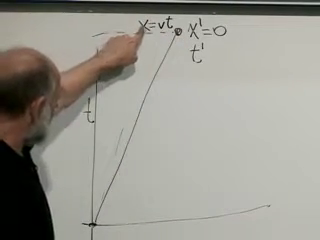
\includegraphics[width=0.72\textwidth]{lecture_04_figure_03.png}\caption{Der bewegte Ursprung: $x=vt$, $x'=0$ und die $t'$-Achse sind drei Beschreibungen derselben Weltlinie.}\lectureframe{00:48:18}\end{figure}

Wenden wir das invariante Intervall auf den gemeinsamen Ursprung und einen späteren Punkt auf dieser Weltlinie an:
\begin{align}
t'^2-x'^2&=t^2-x^2,\\
t'^2&=t^2-v^2t^2,\\
t'&=t\sqrt{1-v^2}.
\label{eq:l4-time-dilation-natural}
\end{align}
Mit wieder eingesetztem $c$ ergibt sich
\begin{equation}
\Delta\tau=\Delta t\sqrt{1-\frac{v^2}{c^2}}
=\frac{\Delta t}{\gamma},
\qquad
\gamma=\frac{1}{\sqrt{1-v^2/c^2}}.
\label{eq:l4-time-dilation}
\end{equation}

\begin{figure}[H]\centering
\includegraphics[width=0.73\textwidth]{lecture_04_figure_09.png}\caption{Das Ergebnis zur Zeitdilatation an der Tafel: Die bewegte Uhr misst in Einheiten mit $c=1$ die Eigenzeit $t'=t\sqrt{1-v^2}$.}\lectureframe{00:50:45}\end{figure}

Der ruhende Beobachter sagt, dass die bewegte Uhr langsamer geht. Aufgrund der Reziprozität muss der bewegte Beobachter dasselbe über ruhende Uhren sagen. Das ist kein Widerspruch, denn die beiden Beschreibungen vergleichen unterschiedliche Paare weit voneinander entfernter Ereignisse.

Tatsächlich erfüllt ein konstanter Wert von $t'$ in Gl.~\eqref{eq:l4-lorentz-natural} die Bedingung
\begin{equation}
t-vx=\text{constant}.
\label{eq:l4-simultaneity}
\end{equation}
Die Gleichzeitigkeitslinien des bewegten Beobachters sind gegenüber den horizontalen Linien $t=\text{constant}$ geneigt. Jeder Beobachter nennt eine andere Auswahl weit voneinander entfernter Uhrenanzeigen gleichzeitig. Berücksichtigt man diesen Unterschied, ist die reziproke Verlangsamung der Uhren widerspruchsfrei.

\begin{figure}[H]\centering
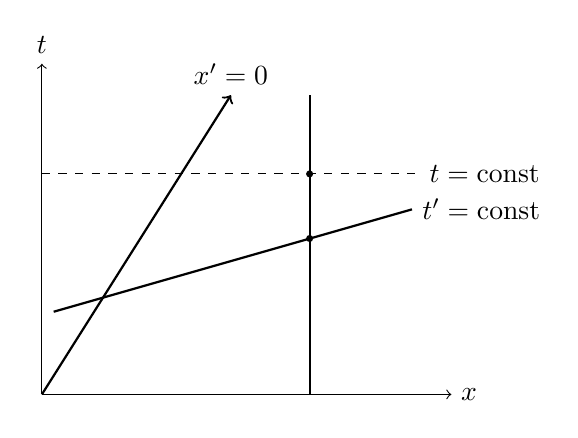
\begin{tikzpicture}[x=1cm,y=1cm]
\draw[->] (0,0) -- (0,4.2) node[above] {$t$};
\draw[->] (0,0) -- (5.2,0) node[right] {$x$};
\draw[thick,->] (0,0) -- (2.4,3.8) node[above] {$x'=0$};
\draw[dashed] (0,2.8) -- (4.8,2.8)
  node[right] {$t=\mathrm{const}$};
\draw[thick] (0.15,1.05) -- (4.7,2.35)
  node[right] {$t'=\mathrm{const}$};
\draw[thick] (3.4,0) -- (3.4,3.8);
\fill (3.4,2.8) circle (0.045);
\fill (3.4,1.98) circle (0.045);
\end{tikzpicture}\caption{Bei der reziproken Zeitdilatation werden Uhrenanzeigen auf unterschiedlichen Gleichzeitigkeitsflächen verglichen.}\end{figure}

\section{Die Wege der Zwillinge}

Zwei Zwillinge beginnen am selben Ereignis. Einer bleibt bei $x=0$. Der andere bewegt sich mit der Geschwindigkeit $v$ nach außen, kehrt um und kommt mit derselben Geschwindigkeit zurück. Bei ihrem Wiedersehen vergleichen sie alle physikalischen Vorgänge, die als Uhr dienen können: Armbanduhren, Herzschlag, Stoffwechsel oder den Alterungsprozess selbst.

Die beiden Reiseabschnitte sollen im Heimatbezugssystem jeweils die Koordinatenzeit $T$ dauern. Die Eigenzeit des zu Hause gebliebenen Zwillings beträgt
\begin{equation}
\tau_{\mathrm{home}}=2T.
\end{equation}
Das Umkehrereignis hat die Koordinaten $(vT,T)$. Der erste Reiseabschnitt trägt daher
\begin{align}
\tau_{\mathrm{leg}}
&=\sqrt{T^2-v^2T^2}
=T\sqrt{1-v^2}.
\end{align}
bei. Der Rückweg trägt denselben Betrag bei, also
\begin{equation}
\tau_{\mathrm{travel}}=2T\sqrt{1-v^2}<2T.
\label{eq:l4-twin}
\end{equation}

\begin{figure}[H]
\centering
\includegraphics[width=0.73\textwidth]{lecture_04_figure_10.png}

\vspace{0.8em}

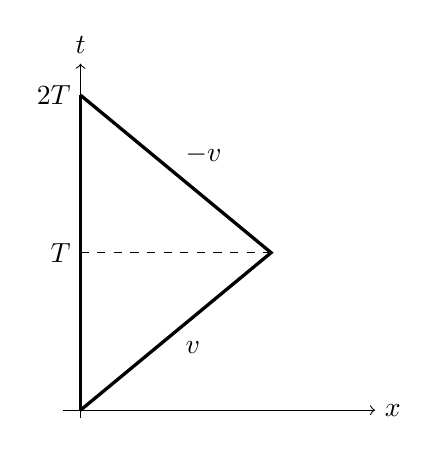
\begin{tikzpicture}[x=1.1cm,y=1cm]
\draw[->] (-0.2,0) -- (3.4,0) node[right] {$x$};
\draw[->] (0,-0.1) -- (0,4.4) node[above] {$t$};
\draw[very thick] (0,0) -- (0,4);
\draw[very thick] (0,0) -- (2.2,2) -- (0,4);
\draw[dashed] (0,2) -- (2.2,2);
\node[left] at (0,2) {$T$};
\node[left] at (0,4) {$2T$};
\node[below right] at (1.1,1.0) {$v$};
\node[above right] at (1.1,3.0) {$-v$};
\end{tikzpicture}\caption{Die Weltlinie des zu Hause gebliebenen Zwillings und die beiden Reiseabschnitte. Ihre Eigenzeiten unterscheiden sich, weil sie verschiedenen Wegen durch die Raumzeit folgen.}\lectureframe{00:59:35}\end{figure}

Die unterschiedlichen Altersangaben sind kein Widerspruch. Der Reiseweg enthält eine Umkehr und ist nicht durch eine einzige Symmetrie zwischen Inertialsystemen mit der geraden Weltlinie des zu Hause gebliebenen Zwillings verknüpft. Auch in der gewöhnlichen euklidischen Geometrie sind die Längen einer geraden Strecke und eines geknickten Weges zwischen zwei Punkten verschieden. In der Minkowski-Geometrie kehrt sich um, welcher Weg das größere Intervall hat; der Vergleich bleibt jedoch geometrisch.

\section{Beschleunigung und die ideale Uhr}

\begin{classroomqa}\audiencequestion{Bei der Umkehr ist die Physik anders, und der Reisende wird beschleunigt. Macht das die Uhrenberechnung ungültig?\lecturetimestamp{01:02:19}}\lecturerresponse{Die Beschleunigung ist real und hilft, die Asymmetrie zu erkennen; man sollte sie nicht wegargumentieren. Die scharfe Ecke ist nur eine idealisierte Zeichnung und lässt sich durch eine endliche Umkehr mit abgerundetem Verlauf ersetzen. Hinzu kommt die physikalische Annahme, dass eine hinreichend kleine, gut gebaute Uhr gegenüber mäßiger Beschleunigung unempfindlich ist und weiterhin die Eigenzeit anzeigt. Eine große oder empfindliche Uhr kann sich verformen oder kaputtgehen; das wäre jedoch ein Mangel des Mechanismus und nicht des Raumzeitintervalls.}\end{classroomqa}

Diese Annahme über ideale Uhren folgt nicht allein aus der Lorentz-Transformation. Sie wird anhand des Verhaltens tatsächlicher Uhrenmechanismen geprüft. Ein Atom ist eine viel bessere Näherung als eine Uhr, die Hunderte von Meilen groß ist, denn der kompakte Mechanismus lässt sich durch Beschleunigung oder Gravitation schwerer verformen. Die allgemeine Relativitätstheorie beim Namen zu nennen, beseitigt dieses physikalische Problem nicht; man müsste weiterhin wissen, wie der gewählte Mechanismus auf seine Umgebung reagiert.

\begin{classroomqa}\audiencequestion{Lässt sich eine beschleunigte Bahn in kurze Abschnitte zerlegen, für die die Inertialanalyse weiterhin gilt?\lecturetimestamp{01:09:08}}\lecturerresponse{Ja. Man zerlegt die Kurve in kurze, nahezu gerade Abschnitte, berechnet für jeden die Eigenzeit und addiert die Ergebnisse. Das entspricht in der Raumzeit der Bestimmung der Länge einer gewöhnlichen Kurve aus vielen kleinen geraden Strecken. Im Kontinuumslimes gilt für eine Bewegung in der flachen Raumzeit, beschrieben in einem Inertialkoordinatensystem,
\[
\tau=\int \sqrt{1-\frac{v(t)^2}{c^2}}\,dt,
\]}\end{classroomqa}

\section{Was die Zwillinge sehen}

Die endgültigen Uhrenanzeigen lassen sich durch das Aussenden von Lichtblitzen operational zugänglich machen. Auf beiden Weltlinien markiert man Intervalle von einer Sekunde Eigenzeit und lässt jeden Zwilling bei jeder Markierung einen Lichtblitz aussenden. Während des Hinwegs treffen die vom jeweils anderen Zwilling empfangenen Blitze in größeren Abständen ein. Auf dem Rückweg kommen sie gehäuft an. Das ist der relativistische Doppler-Effekt, direkt im Raumzeitdiagramm dargestellt.

\begin{figure}[H]\centering
\includegraphics[width=0.73\textwidth]{lecture_04_figure_11.png}\caption{Zwischen der Weltlinie des zu Hause gebliebenen und der des reisenden Zwillings ausgetauschte Lichtsignale. Die größeren Abstände der empfangenen Blitze auf dem Hinweg und ihre Verdichtung auf dem Rückweg erklären jeden ausgesandten Blitz.}\lectureframe{01:12:55}\end{figure}

Keine Bezugssysteme verschwinden aus der Darstellung. Jeder Beobachter empfängt schließlich alle Blitze, die der andere ausgesandt hat; die Empfangsrate hängt jedoch von der Relativbewegung ab. Für die beiden Wege wirken Rotverschiebung auf dem Hinweg und Blauverschiebung auf dem Rückweg unterschiedlich lange. Daher stimmt die Zählung aller empfangenen Blitze mit dem Vergleich der Eigenzeiten überein.

\begin{classroomqa}\audiencequestion{Wenn der zurückkehrende Reisende blauverschobenes Licht empfängt, könnte er dann mehr Energie erhalten, als die Quelle ausgesandt hat?\lecturetimestamp{01:13:50}}\lecturerresponse{Diese Frage erfordert die relativistische Definition der Energie und die Berücksichtigung ihrer Abhängigkeit vom Bezugssystem; beides wurde noch nicht entwickelt. Die Frage ist berechtigt, doch Koordinaten und die Anzahl der Lichtblitze reichen allein nicht aus, um die Energiebilanz zu klären, insbesondere für einen beschleunigten Beobachter. Die Antwort sollte daher aufgeschoben und nicht erraten werden.}\end{classroomqa}

\section{Eine geschlossene räumliche Richtung}

\begin{classroomqa}\audiencequestion{Angenommen, eine räumliche Richtung sei kompakt. Könnte sich ein Zwilling gleichförmig auf ihr bewegen, zum Ausgangsort zurückkehren und dabei jede Beschleunigung vermeiden? Was würde die Zwillinge dann unterscheiden?\lecturetimestamp{01:15:14}}\lecturerresponse{Der Raum ist intrinsisch als Zylinder vorzustellen, nicht als Fläche, die in einen größeren Raum hineingebogen ist; eine radiale Beschleunigung muss es nicht geben. Der zurückkehrende Beobachter begegnet dennoch der globalen Tatsache, dass dieselben Orte wiederkehren. Das deutet auf eine Asymmetrie hin, doch eine vollständige Antwort erfordert eine sorgfältige Behandlung der speziellen Relativitätstheorie mit dieser räumlichen Identifikation. Die Frage bleibt hier offen, statt spontan beantwortet zu werden.}\end{classroomqa}

\begin{figure}[H]
\centering
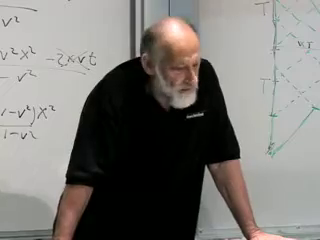
\includegraphics[width=0.72\textwidth]{lecture_04_figure_04.png}

\vspace{0.8em}

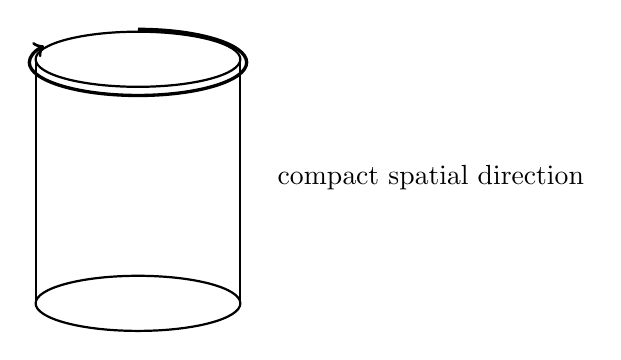
\begin{tikzpicture}[x=1cm,y=1cm]
\draw[thick] (0,0) ellipse (1.3 and 0.35);
\draw[thick] (-1.3,0) -- (-1.3,-3.1);
\draw[thick] (1.3,0) -- (1.3,-3.1);
\draw[thick] (0,-3.1) ellipse (1.3 and 0.35);
\draw[->,very thick] (0.0,0.38) arc (90:-210:1.38 and 0.42);
\node[right] at (1.65,-1.5) {compact spatial direction};
\end{tikzpicture}\caption{Die Frage zum kompakten Raum, wie an der Tafel gezeichnet, mit einem sauberen intrinsischen Zylinder. Es geht um eine globale Identifikation, nicht um Bewegung auf einem Zylinder, der in eine zusätzliche radiale Dimension eingebettet ist.}\lectureframe{01:17:56}\end{figure}

\section{Längen werden auf einer Gleichzeitigkeitsfläche gemessen}

Bei einem Problem der speziellen Relativitätstheorie zeichnet man zuerst das Raumzeitbild. Betrachten wir einen Meterstab, der im ungestrichenen Bezugssystem ruht und dessen Endpunkte bei $x=0$ und $x=1$ liegen. Mit der Zeit zeichnen seine beiden Endpunkte vertikale Weltlinien. Der Stab überstreicht ein Band in der Raumzeit.

Der bewegte Beobachter muss beide Endpunkte bei demselben Wert der bewegten Zeit $t'$ messen. Aus Gl.~\eqref{eq:l4-simultaneity} folgt, dass die Fläche durch den Ursprung mit $t'=0$ die Bedingung
\begin{equation}
t=vx
\end{equation}
erfüllt, in Einheiten mit $c=1$. Sie schneidet die Weltlinie des rechten Endpunkts $x=1$ bei $t=v$.

\begin{figure}[H]
\centering
\includegraphics[width=0.73\textwidth]{lecture_04_figure_12.png}

\vspace{0.8em}

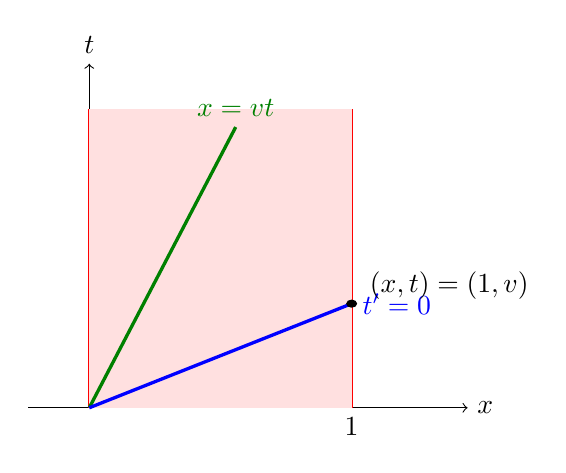
\begin{tikzpicture}[x=1.55cm,y=1.15cm]
\draw[->] (-0.5,0) -- (3.1,0) node[right] {$x$};
\draw[->] (0,0) -- (0,3.8) node[above] {$t$};
\draw[very thick,red] (0,0) -- (0,3.3);
\draw[very thick,red] (2.15,0) -- (2.15,3.3);
\fill[red!12] (0,0) rectangle (2.15,3.3);
\draw[very thick,green!50!black] (0,0) -- (1.2,3.1)
  node[above] {$x=vt$};
\draw[very thick,blue] (0,0) -- (2.15,1.15)
  node[right] {$t'=0$};
\fill (2.15,1.15) circle (0.045);
\node[right] at (2.22,1.35) {$(x,t)=(1,v)$};
\node[below] at (2.15,0) {$1$};
\end{tikzpicture}\caption{Ein ruhender Stab überstreicht ein Band in der Raumzeit. Die vom bewegten Beobachter gemessene Länge ist der Abstand zwischen seinen Endpunkten auf einer Fläche mit konstantem $t'=\mathrm{const}$.}\lectureframe{01:24:20}\end{figure}

Der gewählte Abstand zwischen den Endpunkten ist raumartig; daher verwendet man die positive räumliche Form der Invariante:
\begin{equation}
x'^2-t'^2=x^2-t^2.
\end{equation}
Am gewählten Endpunkt gilt $t'=0$, $x=1$ und $t=v$. Somit
\begin{align}
x'^2&=1-v^2,\\
x'&=\sqrt{1-v^2}.
\end{align}
Eine Ruhelänge $L$ wird im bewegten Bezugssystem also als
\begin{equation}
L'=L\sqrt{1-v^2/c^2}=\frac{L}{\gamma}.
\label{eq:l4-length-contraction}
\end{equation}
gemessen.

\begin{figure}[H]\centering
\includegraphics[width=0.76\textwidth]{lecture_04_figure_13.png}\caption{Die vollständige Herleitung der Längenkontraktion und das Ergebnis an der Tafel $x'=\sqrt{1-v^2}$ für eine Ruhelänge von einer Einheit.}\lectureframe{01:28:10}\end{figure}

Auch die reziproke Aussage gilt: Der Beobachter auf dem Bahnsteig schreibt dem längs ausgerichteten Meterstab im Zug eine kürzere Länge zu. Wieder wählen die beiden Beobachter unterschiedliche gleichzeitige Ereignisse an den Endpunkten; daher ist die Reziprozität kein Widerspruch.

\section{Fragen zum Abschluss}

\begin{classroomqa}\audiencequestion{Breitet sich außer Licht noch etwas mit Lichtgeschwindigkeit aus? Was ist insbesondere mit der Gravitation?\lecturetimestamp{01:29:29}}\lecturerresponse{Die allgemeine Relativitätstheorie sagt Gravitationswellen voraus, die sich mit $c$ ausbreiten. Zum Zeitpunkt dieser Vorlesung stammten die Belege indirekt aus Systemen wie Doppelsternpulsaren; Gravitationswellen waren noch nicht direkt nachgewiesen worden.\editorialnote{Die experimentelle Lage änderte sich nach dieser Vorlesung von 2006. LIGO wies GW150914 im Jahr 2015 direkt nach, und die gemeinsame Beobachtung von GW170817 und seinem elektromagnetischen Gegenstück im Jahr 2017 zeigte, dass die Ausbreitungsgeschwindigkeiten von Gravitation und Licht bis auf wenige Teile von $10^{15}$ übereinstimmen. Siehe \url{https://ligo.org/detections/gw150914/} und \url{https://doi.org/10.1103/PhysRevLett.119.251302}.}}\end{classroomqa}

\begin{classroomqa}\audiencequestion{Kann ein Astronaut eine Entfernung von vielen Lichtjahren in weniger Eigenzeit durchqueren, als die in Lichtjahren angegebene Entfernung beträgt? Würde das bedeuten, dass er sich schneller als Licht bewegt?\lecturetimestamp{01:30:38}}\lecturerresponse{Die Eigenzeit des Astronauten beträgt $\sqrt{\Delta t^2-\Delta x^2}$; sie ist kleiner als die Koordinatenzeit $\Delta t$. Im Inertialsystem des Astronauten ist der Abstand zwischen den Sternen lorentzkontrahiert. Die Sterne bewegen sich mit der Geschwindigkeit $-v$, nicht schneller als Licht; es ist schlicht eine kürzere, kontrahierte Strecke zu durchqueren.}\end{classroomqa}

Beginnt der Astronaut aus dem Ruhezustand und beschleunigt, ändert sich die Beschreibung von einem momentanen Inertialsystem zum nächsten. Der den Sternen zugewiesene Abstand kann sich während dieses Übergangs ändern. Man kann nicht eine einzige feste Lorentz-Transformation auf die gesamte beschleunigte Geschichte anwenden; die gesamte Eigenzeit ergibt sich dennoch durch Addition der Beiträge entlang der Weltlinie. Dasselbe gilt für einen realistischen Zwilling, der startet, umkehrt und abbremst, statt mit Reisegeschwindigkeit geboren zu werden.

\begin{classroomqa}\audiencequestion{Entstehen diese Rätsel dadurch, dass die Zeit als etwas Besonderes behandelt wird? Müssen wir sie eine vierte Dimension nennen?\lecturetimestamp{01:36:43}}\lecturerresponse{Man muss nicht mit dem Schlagwort beginnen, die Zeit sei eine vierte Dimension. Die Lorentz-Transformation selbst erzwingt eine Vermischung von Raum und Zeit, während das Intervall $t^2-x^2-y^2-z^2$ sie als Bestandteile einer einzigen Geometrie auffasst, wobei für Zeit und Raum unterschiedliche Vorzeichen gelten. Bei niedriger Geschwindigkeit wird die Vermischung vernachlässigbar, und die vertraute Newtonsche Intuition kehrt zurück. Bei relativistischen Geschwindigkeiten lassen sich Raum und Zeit jedoch nicht als grundsätzlich entkoppelt betrachten.}\end{classroomqa}

Zeitdilatation, Längenkontraktion, der Vergleich der Zwillinge und die verkürzte Reisezeit sind also keine voneinander unabhängigen Tricks. Sie folgen alle aus drei Vorgehensweisen: die verglichenen Ereignisse bestimmen, ihre Raumzeitgeometrie zeichnen und das invariante Intervall verwenden.